\subsection*{KDD}

\begin{figure}[!htp]
	\centering
	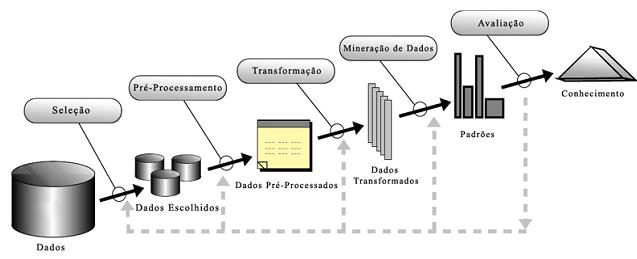
\includegraphics[scale=.65]{../img/kdd/pt.png}
	\caption{Ilustração das etapas da extração de conhecimento}
	\label{img:kdd}
\end{figure}

\begin{enumerate}
	\item \underline{Dados:}
	      conjunto de dados organizados de forma \textit{qualitativa} ou \textit{quantitativa} sobre determinado tema, no qual possibilidade a extração de informação que pode resultar em conhecimento.
	\item \underline{Pré-processamento dos dados:}
	      Selecionar os dados de acordo com a demanda do estudo, descartando assim dados irrelevantes, a fim de tornar a análise dos eficiente e eficaz.
	      As etapas são distribuídas:
	      \begin{itemize}
		      \item \underline{limpeza:} remoção de ruídos de dados inconsistentes e ausentes;
		      \item \underline{integração:}combinação dos dados de diferentes fontes;
		      \item \underline{seleção:} escolha de dados relevantes à análise; e
		      \item \underline{transformação:} consolidação dos dados em formato apropriado.
	      \end{itemize}
	\item \underline{Mineração de dados:}
	      Utilização de métricas e medidas estatísticas, para representar o conjunto de dados e a sua distribuição.
	      Tais medidas são análise descritiva, agrupamento, predição, associação e detecção de anomalias.
	\item underline{Avaliação:}
	      Identificar os padrões obtidos pela representação do conhecimento são válidos, ou seja, representativo.
\end{enumerate}
